\chapter{Testy Funkcjonalne}
\section{Wstęp}
\section{Eliminacja zakłóceń sinusoidalnych}
\subsection{Integracja bloku filtra w projekcie}
\begin{figure}[ht]
\centering
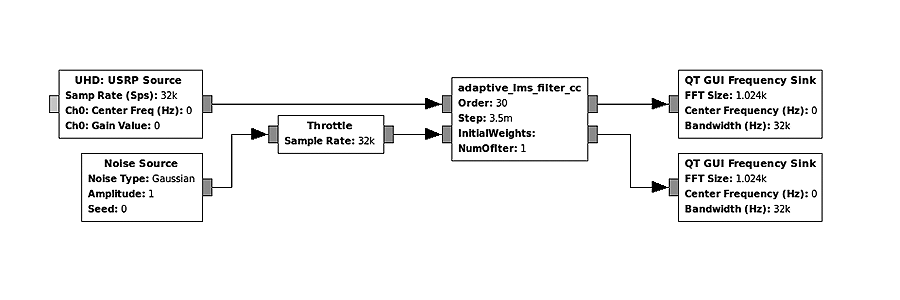
\includegraphics[scale=1.1]{ch5_integration.png}
\end{figure}
\begin{figure}[ht]
\centering
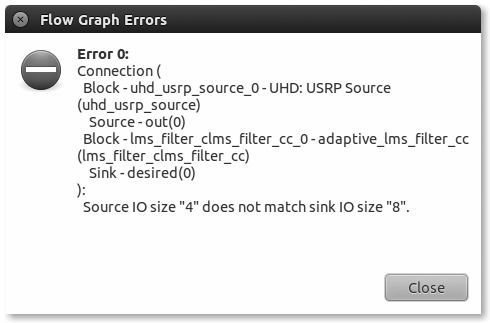
\includegraphics[scale=0.7]{ch5_error.png}
\end{figure}
\subsection{Weryfikacja poprawności działania}
\section{Korekcja adaptacyjna}

\begin{sidewaystable}[t]
\centering
\caption{My caption3}
\label{my-label3}
\begin{tabular}{l}
\hline
Transmisja bez korekcji \\
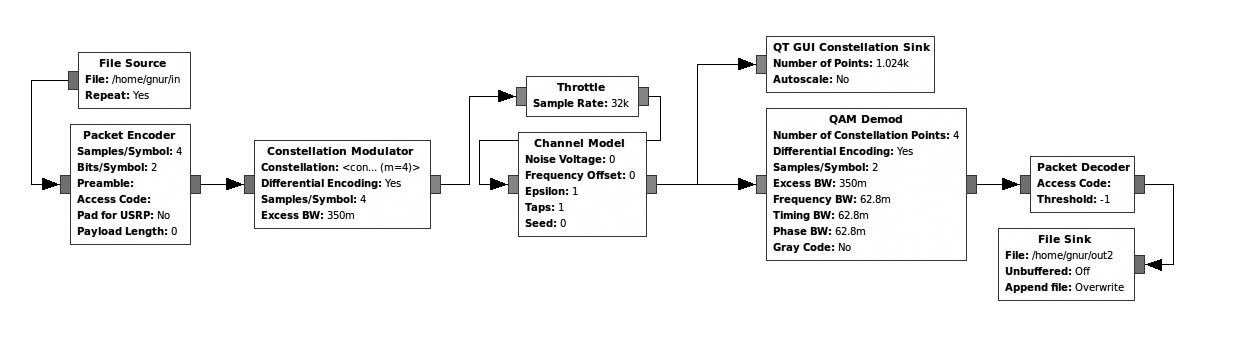
\includegraphics[scale=0.5]{noeq.png}\\ \hline
Transmisja z korekcją   \\
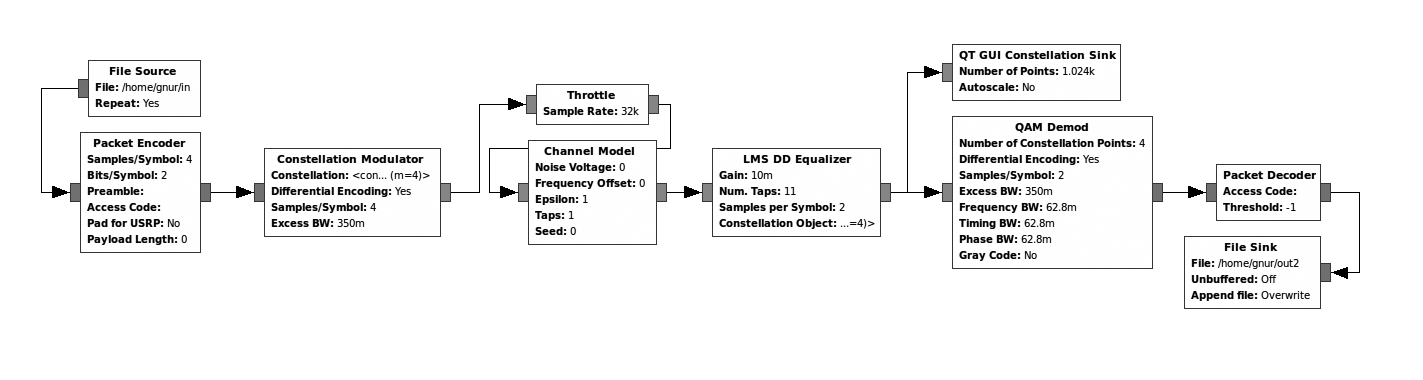
\includegraphics[scale=0.5]{eq.png}\\
\end{tabular}
\end{sidewaystable}

\begin{table}
\centering
\caption{My caption}
\label{my-label2}
\begin{tabular}{|l|l|l|}
\hline
0mV      & 150mV    & 200mV    \\
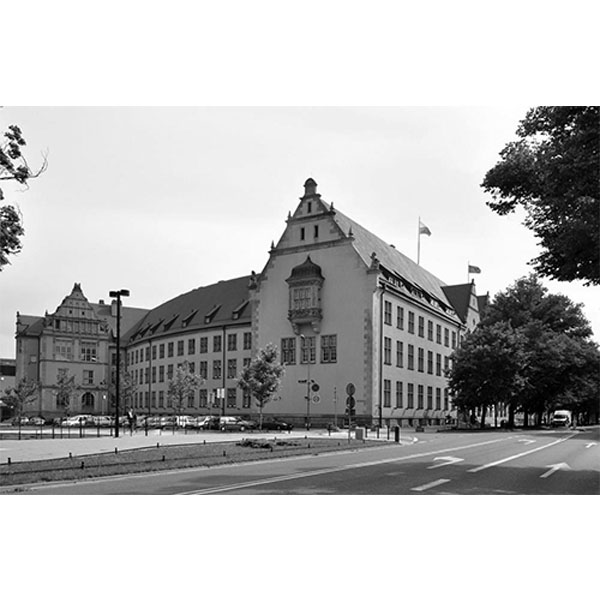
\includegraphics[scale=0.45]{a1origin} & 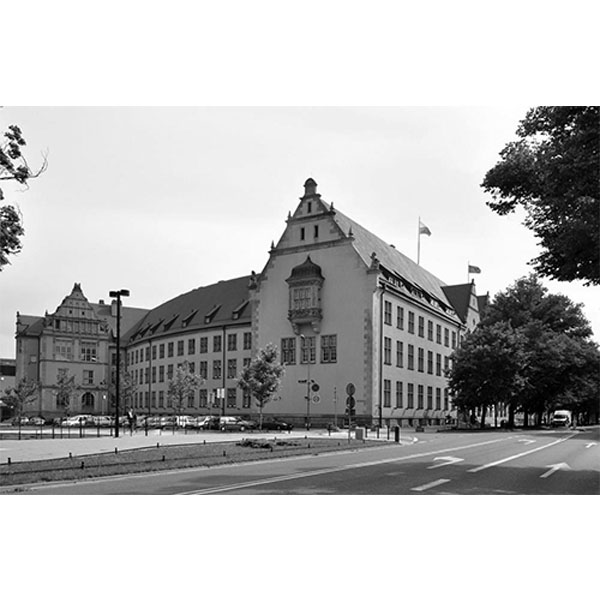
\includegraphics[scale=0.45]{a1origin} & 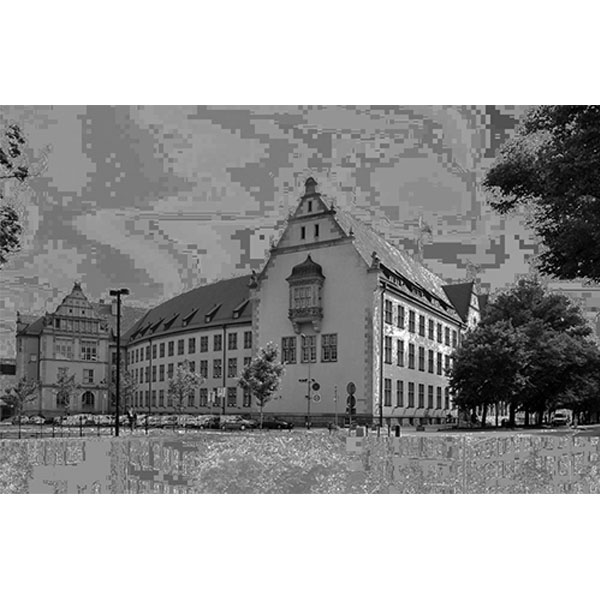
\includegraphics[scale=0.45]{noeq200mva1} \\
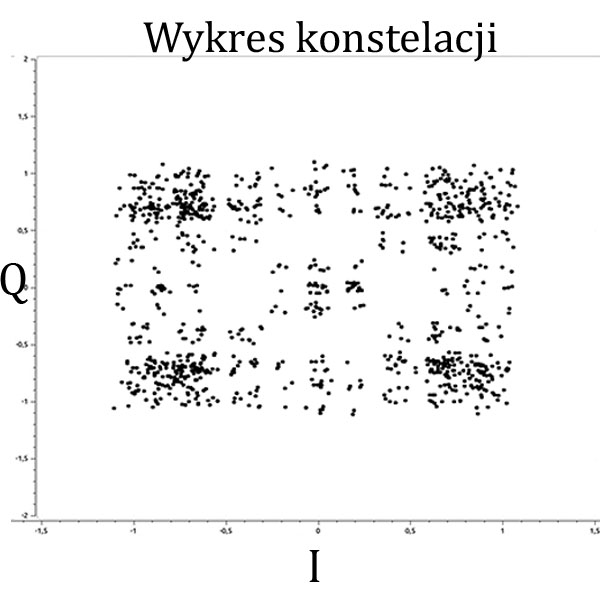
\includegraphics[scale=0.45]{noeq0mv}   & 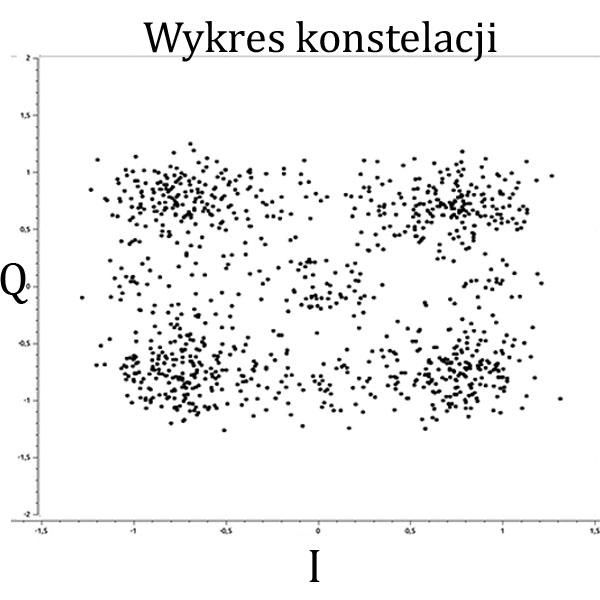
\includegraphics[scale=0.45]{noeq150mv}   & 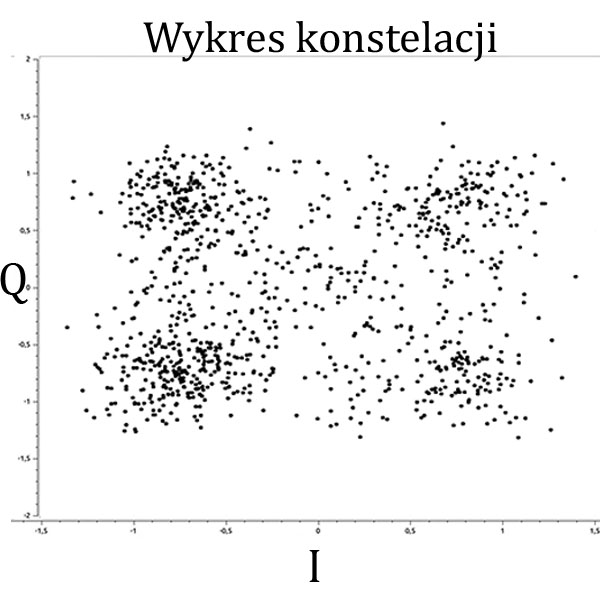
\includegraphics[scale=0.45]{noeq200mv}  \\ \hline
\end{tabular}
\end{table}


\begin{table}
\centering
\caption{My caption}
\label{my-label}
\begin{tabular}{|l|l|l|}
\hline
0mV      & 200mV    & 250mV    \\
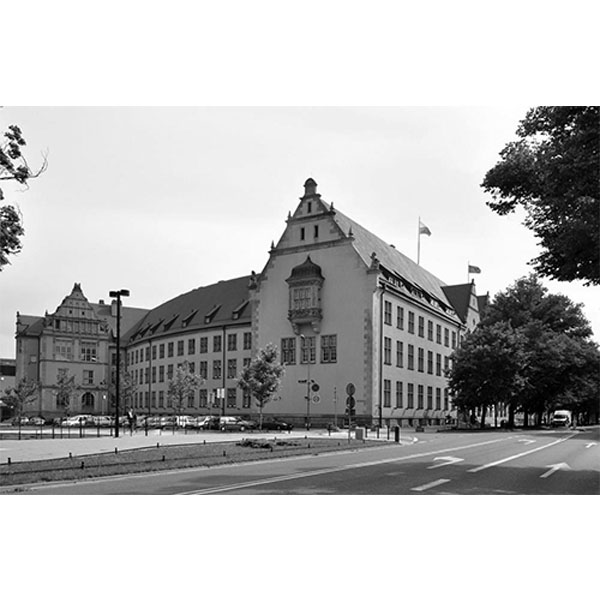
\includegraphics[scale=0.45]{a1origin} & 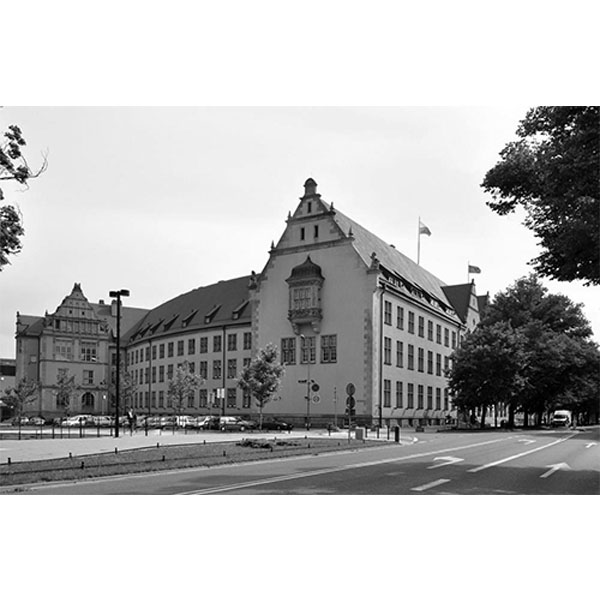
\includegraphics[scale=0.45]{a1origin} & 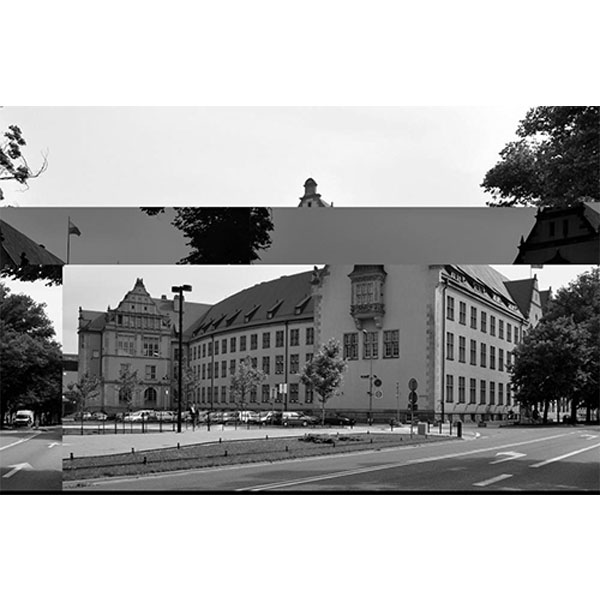
\includegraphics[scale=0.45]{eq250mva1} \\
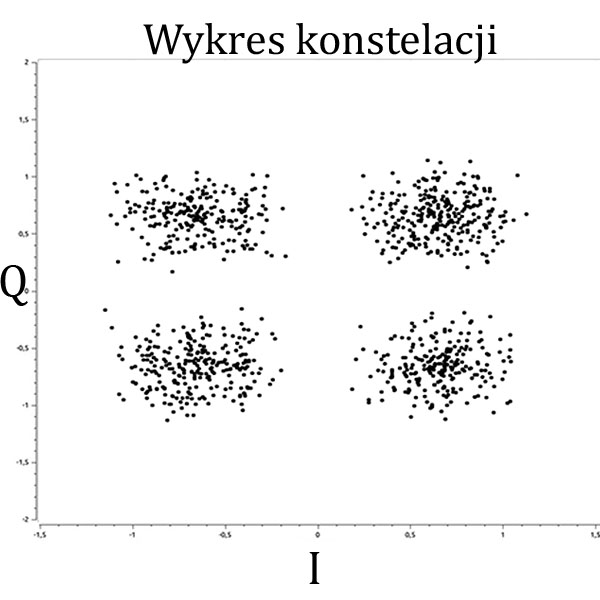
\includegraphics[scale=0.45]{eq0mv}   & 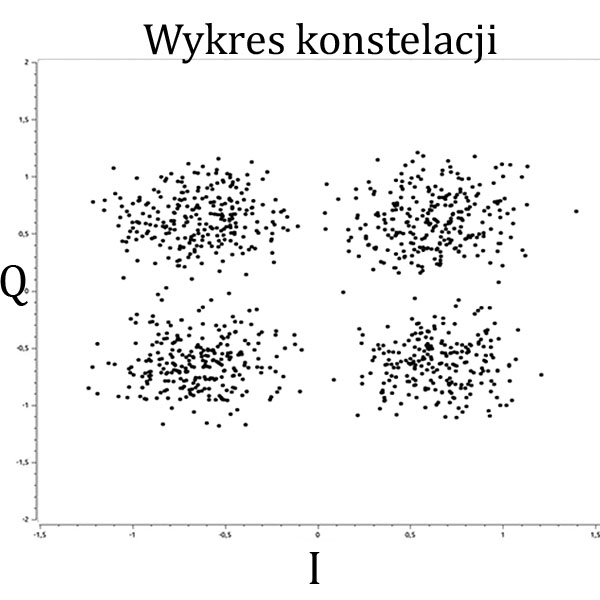
\includegraphics[scale=0.45]{eq200mv}   & 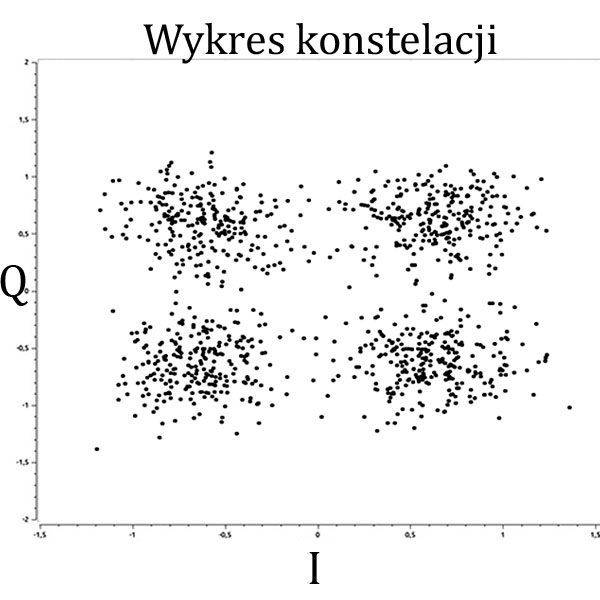
\includegraphics[scale=0.45]{eq250mv}  \\ \hline
\end{tabular}
\end{table}




